\documentclass{Configuration_Files/PoliMi3i_thesis}

%------------------------------------------------------------------------------
%	REQUIRED PACKAGES AND  CONFIGURATIONS
%------------------------------------------------------------------------------

% CONFIGURATIONS
\usepackage{parskip} % For paragraph layout
\usepackage{setspace} % For using single or double spacing
\usepackage{emptypage} % To insert empty pages
\usepackage{multicol} % To write in multiple columns (executive summary)
\setlength\columnsep{15pt} % Column separation in executive summary
\setlength\parindent{0pt} % Indentation
\raggedbottom
\usepackage{multirow}

% PACKAGES FOR TITLES
\usepackage{titlesec}
% \titlespacing{\section}{left spacing}{before spacing}{after spacing}
\titlespacing{\section}{0pt}{3.3ex}{2ex}
\titlespacing{\subsection}{0pt}{3.3ex}{1.65ex}
\titlespacing{\subsubsection}{0pt}{3.3ex}{1ex}
\usepackage{color}

% PACKAGES FOR LANGUAGE AND FONT
\usepackage[english]{babel} % The document is in English  
\usepackage[utf8]{inputenc} % UTF8 encoding
\usepackage[T1]{fontenc} % Font encoding
\usepackage[11pt]{moresize} % Big fonts

% PACKAGES FOR IMAGES
\usepackage{graphicx}
\usepackage{transparent} % Enables transparent images
\usepackage{eso-pic} % For the background picture on the title page
\usepackage{subfig} % Numbered and caption subfigures using \subfloat.
\usepackage{tikz} % A package for high-quality hand-made figures.
\usetikzlibrary{}
\graphicspath{{./Images/}} % Directory of the images
\usepackage{caption} % Coloured captions
\usepackage{xcolor} % Coloured captions
\usepackage{amsthm,thmtools,xcolor} % Coloured "Theorem"
\usepackage{float}

% STANDARD MATH PACKAGES
\usepackage{amsmath}
\usepackage{amsthm}
\usepackage{amssymb}
\usepackage{amsfonts}
\usepackage{bm}
\usepackage[overload]{empheq} % For braced-style systems of equations.
\usepackage{fix-cm} % To override original LaTeX restrictions on sizes

% PACKAGES FOR TABLES
\usepackage{tabularx}
\usepackage{longtable} % Tables that can span several pages
\usepackage{colortbl}

% PACKAGES FOR ALGORITHMS (PSEUDO-CODE)
\usepackage{algorithm}
\usepackage{algorithmic}

% PACKAGES FOR REFERENCES & BIBLIOGRAPHY
\usepackage[colorlinks=true,linkcolor=black,anchorcolor=black,citecolor=black,filecolor=black,menucolor=black,runcolor=black,urlcolor=black]{hyperref} % Adds clickable links at references
\usepackage{cleveref}
\usepackage[square, numbers, sort&compress]{natbib} % Square brackets, citing references with numbers, citations sorted by appearance in the text and compressed
\bibliographystyle{abbrvnat} % You may use a different style adapted to your field

% OTHER PACKAGES
\usepackage{pdfpages} % To include a pdf file
\usepackage{afterpage}
\usepackage{lipsum} % DUMMY PACKAGE
\usepackage{fancyhdr}
\usepackage{wasysym} % For the headers
\usepackage{rotating}
\usepackage{listings}
\usepackage{hyperref}
%%
% Alloy language definition for using with the listings package.
%
% 2017, Daniel Andrade
% BSD 3-Clause License
%%
\lstdefinelanguage{alloy}{
    morekeywords={
        module, open, as,
        private, abstract, sig, extends, in,
        lone, some, one, disj,
        fact, pred, fun, assert,
        run, check,
        for, but, exactly,
        this, not, implies, else, let,
        not, no, set, all, sum,
        iff, or, Int, and,
        none, univ, iden
    },
    sensitive=true,
    morecomment=[l]{//},
    morecomment=[l]{--},
    morecomment=[s]{/*}{*/},
    morestring=[b]{"},
%literate={->}{$\rightarrow$}1
% replacing characters can cause problems when copying from PDF to editor
}[keywords,comments,strings]
\fancyhf{}

% Input of configuration file. Do not change config.tex file unless you really know what you are doing. 
% Define blue color typical of polimi
\definecolor{bluepoli}{cmyk}{0.4,0.1,0,0.4}

% Custom theorem environments
\declaretheoremstyle[
  headfont=\color{bluepoli}\normalfont\bfseries,
  bodyfont=\color{black}\normalfont\itshape,
]{colored}

% Set-up caption colors
\captionsetup[figure]{labelfont={color=bluepoli}} % Set colour of the captions
\captionsetup[table]{labelfont={color=bluepoli}} % Set colour of the captions
\captionsetup[algorithm]{labelfont={color=bluepoli}} % Set colour of the captions

\theoremstyle{colored}
\newtheorem{theorem}{Theorem}[chapter]
\newtheorem{proposition}{Proposition}[chapter]

% Enhances the features of the standard "table" and "tabular" environments.
\newcommand\T{\rule{0pt}{2.6ex}}
\newcommand\B{\rule[-1.2ex]{0pt}{0pt}}

% Pseudo-code algorithm descriptions.
\newcounter{algsubstate}
\renewcommand{\thealgsubstate}{\alph{algsubstate}}
\newenvironment{algsubstates}
  {\setcounter{algsubstate}{0}%
   \renewcommand{\STATE}{%
     \stepcounter{algsubstate}%
     \Statex {\small\thealgsubstate:}\space}}
  {}

% New font size
\newcommand\numfontsize{\@setfontsize\Huge{200}{60}}

% Title format: chapter
\titleformat{\chapter}[hang]{
\fontsize{50}{20}\selectfont\bfseries\filright}{\textcolor{bluepoli} \thechapter\hsp\hspace{2mm}\textcolor{bluepoli}{|   }\hsp}{0pt}{\huge\bfseries \textcolor{bluepoli}
}

% Title format: section
\titleformat{\section}
{\color{bluepoli}\normalfont\Large\bfseries}
{\color{bluepoli}\thesection.}{1em}{}

% Title format: subsection
\titleformat{\subsection}
{\color{bluepoli}\normalfont\large\bfseries}
{\color{bluepoli}\thesubsection.}{1em}{}

% Title format: subsubsection
\titleformat{\subsubsection}
{\color{bluepoli}\normalfont\large\bfseries}
{\color{bluepoli}\thesubsubsection.}{1em}{}

% Shortening for setting no horizontal-spacing
\newcommand{\hsp}{\hspace{0pt}}

\makeatletter
% Renewcommand: cleardoublepage including the background pic
\renewcommand*\cleardoublepage{%
  \clearpage\if@twoside\ifodd\c@page\else
  \null
  \AddToShipoutPicture*{\BackgroundPic}
  \thispagestyle{empty}%
  \newpage
  \if@twocolumn\hbox{}\newpage\fi\fi\fi}
\makeatother

%For correctly numbering algorithms
\numberwithin{algorithm}{chapter}

\definecolor{dkgreen}{rgb}{0,0.6,0}
\definecolor{gray}{rgb}{0.5,0.5,0.5}
\definecolor{mauve}{rgb}{0.58,0,0.82}

\lstset{frame=tb,
    language=alloy,
    aboveskip=3mm,
    belowskip=3mm,
    showstringspaces=false,
    columns=flexible,
    basicstyle={\small\ttfamily},
    numbers=none,
    numberstyle=\tiny\color{gray},
    keywordstyle=\bf\color{blue},
    commentstyle=\it\color{dkgreen},
    stringstyle=\color{mauve},
    breaklines=true,
    breakatwhitespace=true,
    tabsize=3
}

%----------------------------------------------------------------------------
%	NEW COMMANDS DEFINED
%----------------------------------------------------------------------------



% EXAMPLES OF NEW COMMANDS
%\newcommand{\bea}{\begin{eqnarray}} % Shortcut for equation arrays
%\newcommand{\eea}{\end{eqnarray}}
%\newcommand{\e}[1]{\times 10^{#1}}  % Powers of 10 notation

%----------------------------------------------------------------------------
%	ADD YOUR PACKAGES (be careful of package interaction)
%----------------------------------------------------------------------------

%----------------------------------------------------------------------------
%	ADD YOUR DEFINITIONS AND COMMANDS (be careful of existing commands)
%----------------------------------------------------------------------------

%----------------------------------------------------------------------------
%	BEGIN OF YOUR DOCUMENT
%----------------------------------------------------------------------------

\begin{document}

    \fancypagestyle{plain}{%
    \fancyhf{} % Clear all header and footer fields
    \fancyhead[RO,RE]{\thepage} %RO=right odd, RE=right even
    \renewcommand{\headrulewidth}{0pt}
    \renewcommand{\footrulewidth}{0pt}}

%----------------------------------------------------------------------------
%	TITLE PAGE
%----------------------------------------------------------------------------

    \pagestyle{empty} % No page numbers
    \frontmatter % Use roman page numbering style (i, ii, iii, iv...) for the preamble pages
    
    \puttitle{
            title=Software Engineering 2\\Requirements Analysis and\\Specification Document,
            name1=De Matteis Alessandro - 10845281,
            name2=Marino Margherita - 10795242,
            name3=Monaco Giorgio - 10775329,
            academicyear=2024-2025,
            version=1.0,
            releasedate=22/12/2024,
    } % These info will be put into your Title page 

%----------------------------------------------------------------------------
%	PREAMBLE PAGES: ABSTRACT (inglese e italiano), EXECUTIVE SUMMARY
%----------------------------------------------------------------------------
    \startpreamble
    \setcounter{page}{1} % Set page counter to 1


%----------------------------------------------------------------------------
%	LIST OF CONTENTS/FIGURES/TABLES/SYMBOLS
%----------------------------------------------------------------------------

% TABLE OF CONTENTS
    \thispagestyle{empty}
    \tableofcontents % Table of contents 
    \thispagestyle{empty}
    \cleardoublepage
    
%-------------------------------------------------------------------------
%	THESIS MAIN TEXT
%-------------------------------------------------------------------------
% In the main text of your thesis you can write the chapters in two different ways:
%
%(1) As presented in this template you can write:
%    \chapter{Title of the chapter}
%    *body of the chapter*
%
%(2) You can write your chapter in a separated .tex file and then include it in the main file with the following command:
%    \chapter{Title of the chapter}
%    \input{chapter_file.tex}
%
% Especially for long thesis, we recommend you the second option.

    \addtocontents{toc}{\vspace{2em}} % Add a gap in the Contents, for aesthetics
    \mainmatter % Begin numeric (1,2,3...) page numbering

% --------------------------------------------------------------------------
% NUMBERED CHAPTERS % Regular chapters following
% --------------------------------------------------------------------------

    \chapter{Introduction}
    \label{ch:introduction}%
    \section{Purpose}
\label{sec:purpose}%

As the demand for skilled graduates grows, bridging the gap between academic learning and practical industry experience has become essential. However, students often face challenges in finding internships that align with their skills and career goals, while companies struggle to identify candidates who truly match their specific needs. Traditional job boards often fail to meet the specific needs of internships, causing mismatches and missed opportunities for students and employers.
Students and companies (S\&C) exists to address this gap by providing a tailored matchmaking platform. By aligning students’ skills, experiences, and aspirations with detailed internship roles, S\&C ensures better fit and smoother transitions into the workforce. The platform supports proactive searches, personalized recommendations, and structured selection processes, ultimately helping students gain hands-on experience while allowing companies to find the right talent for their projects.


\subsection{Goals}
\label{subsec:goals}%

\newcounter{g}
\setcounter{g}{1}
\newcommand{\cg}{\theg\stepcounter{g}}
\textbf{[G\cg]:} University students would like to find internships that better
align with their interests and field of study.

\textbf{[G\cg]:} Companies would like to offer internships to students who best
match the related figure.

\textbf{[G\cg]:} Improve communication and coordination between students and
companies in the selection process.

\textbf{[G\cg]:} Evolve the recommendation system through feedback and
suggestions (provided by students and companies) to improve future
matches.

\textbf{[G\cg]:} Universities would like to monitor internships and handle any
emerging issues promptly, ensuring a smooth and beneficial experience
for all parties involved.

\section{Scope}
\label{sec:scope}%

In this section, we are going to identify the S\&C platform domain. There are three main users that interact with the system:

\begin{itemize}
\item
  \textbf{Students} -- University students seeking internships as part of their academic or career development. They can use S\&C to
  proactively browse available internships, receive customized recommendations based on their profiles, and interact with companies to begin the application and selection process.
\item
  \textbf{Companies} -- Businesses and organizations that offer internships. These companies use S\&C to advertise internship roles with detailed information on project tasks, required skills, technologies, and benefits. S\&C enables companies to receive suitable student profiles automatically, simplifying their candidate search and supporting the structured interview and selection process.
\item
  \textbf{Universities} -- Academic institutions that need to monitor and oversee their students' internship experiences. Universities use S\&C to track the status and progress of internships, address student concerns, and intervene in issues that may impact the quality of the internship.
\end{itemize}

According to the World and Machine paradigm we can identify the Machine as the System to be developed and the environment in which S\&C will be used as the World. This separation allows us to classify the entire phenomena in three different types.

\subsection{World Phenomena}
\label{subsec:world_phenomena}%

Events that take place in the real world and that the machine cannot observe:

\newcounter{w}
\setcounter{w}{1}
\newcommand{\cw}{\thew\stepcounter{w}}
\textbf{[WP\cw]:} The company creates and defines internship opportunities independently, describing tasks, required skills, and terms.

\textbf{[WP\cw]:} The student creates CVs detailing his skills and attitudes.

\textbf{[WP\cw]:} The company conducts an interview with the student.

\textbf{[WP\cw]:} The student wants to accept/reject the proposal.

\textbf{[WP\cw]:} The student or the company encounters problems during the internship and wants to report it.

\textbf{[WP\cw]:} The university handles the complaint submitted by his student or a related company.

\subsection{Machine Phenomena}
\label{subsec:machine_phenomena}%

Events that take place inside the System and cannot be observed by the
real world.

\newcounter{m}
\setcounter{m}{1}
\newcommand{\cm}{\them\stepcounter{m}}
\textbf{[MP\cm]:} The internal processes analyzes student profiles and internship postings to generate recommendations.

\textbf{[MP\cm]:} The recommendation system automatically improves using feedback and suggestions.

\subsection{Shared phenomena}
\label{subsec:shared_phenomena}%

\begin{itemize}
\item
  \textbf{World controlled}
\end{itemize}

Controlled by the world and observed by the machine.

\newcounter{s}
\setcounter{s}{1}
\newcommand{\cs}{\thes\stepcounter{s}}
\textbf{[SP\cs]:} The Guest signs up to the system.

\textbf{[SP\cs]:} The User logs in to the system.

\textbf{[SP\cs]:} The C uploads internship terms and details which the system then collects.

\textbf{[SP\cs]:} The S improves/edits his CV based on the suggestions.

\textbf{[SP\cs]:} The C improves/edits his internship insertion based on the suggestions.

\textbf{[SP\cs]:} The S looks for an internship on the platform, by querying a company's name.

\textbf{[SP\cs]:} The S reviews a C's profile.

\textbf{[SP\cs]:} The S reviews his calendar.

\textbf{[SP\cs]:} The S surf through the recommended internships.

\textbf{[SP\cs]:} The S reviews an internship insertion.

\textbf{[SP\cs]:} The S or the C submits feedback and suggestions about the matchmaking process.

\textbf{[SP\cs]:} The S applies for an internship.

\textbf{[SP\cs]:} The C reviews a candidate's profile.

\textbf{[SP\cs]:} The C sends a contact request in order to offer an internship to a recommended student.

\textbf{[SP\cs]:} The S accepts/refuses a contact request by a company.

\textbf{[SP\cs]:} The C and the S schedule an interview through the chat.

\textbf{[SP\cs]:} The S and the C finalize the selection process after the interview.

\textbf{[SP\cs]:} The C offers an internship to the student after the interview.

\textbf{[SP\cs]:} The S accepts/refuses the proposed internship.

\textbf{[SP\cs]:} The S or the C submits problems, complaints and information about the ongoing internship.

\textbf{[SP\cs]:} The U monitors the ongoing internship.

\textbf{[SP\cs]:} The U interrupts the internship. \\

\begin{itemize}
\item
  \textbf{Machine controlled}
\end{itemize}

Controlled by the machine and observed by the World.

\textbf{[SP\cs]:} The system analyzes the CV and suggests to the S how to improve it.

\textbf{[SP\cs]:} The system analyzes the Insertion and suggests to the C how to improve it.

\textbf{[SP\cs]:} The system recommends the best internships to the S based on his CV, his attitudes and previously submitted feedback.

\textbf{[SP\cs]:} The system suggests the best candidates to the company based on matching algorithms and keywords.

\textbf{[SP\cs]:} The system notifies the S when new recommended internships become available by sending an email and a notification.

\textbf{[SP\cs]:} The system notifies the C of potential candidates when new CVs become available by sending an email and a notification.

\textbf{[SP\cs]:} The system asks the S and the company to provide feedback or suggestions about the matchmaking process.

\textbf{[SP\cs]:} The system establishes contact between the S and the C when both parties have accepted each other's request.

\textbf{[SP\cs]:} The system adds to the S\&C calendar the start and the end date of the internship after the contract agreement.

\textbf{[SP\cs]:} The system adds to the S\&C registers in the calendar the submission of information, complaint or problem.


\section{Definitions, Acronyms, Abbreviations}
\label{sec:definition_acronyms_abbreviations}%

\subsection{Definitions}
\label{subsec:definitions}%

\begin{itemize}
\item
  \textbf{Recommendation}: The process of identifying and suggesting internships to students and suitable candidates to companies using keyword searches, statistical analyses, or other matching algorithms.
\item
  \textbf{Selection Process}: A structured process following a contact in which companies interview and assess students to determine fit.
\item
  \textbf{Matching}: The automated or semi-automated process of pairing students with internships based on their profiles and internship requirements.
\item
  \textbf{Feedback}: Information provided by students and companies on the quality of the matchmaking process or the internship experience, used to improve recommendations.
\item
  \textbf{Internship Monitoring}: Ongoing observation on internship status.
\item
  \textbf{Users:} referred to logged-in guests: Universities, Companies and Students.
\item
  \textbf{Guest:} non logged visitors.
\item
  \textbf{S\&C Calendar:} a built-in calendar where all events (start and end date of internship, interviews) are visible and scheduled.
\end{itemize}

\subsection{Acronyms}
\label{subsec:acronyms}%

\begin{itemize}
\item
  \textbf{S\&C}: Students \& Companies.
\item
  \textbf{UI}: User Interface.
\item
  \textbf{API}: Application Programming Interface.
\end{itemize}

\subsection{Abbreviations}
\label{subsec:abbreviations}%

\begin{itemize}
\item
  \textbf{[G*]:} Goal.
\item
  \textbf{[D*]:} Domain Assumption.
\item
  \textbf{[R*]:} Functional Requirement.
\item
  \textbf{[WP*]:} World Phenomena.
\item
  \textbf{[MP*]:} Machine Phenomena.
\item
  \textbf{[SP*]:} Shared Phenomena.
\item
  \textbf{[UC*]:} Use Case.
\item
  \textbf{[S]} Student.
\item
  \textbf{[C]}: Company.
\item
  \textbf{[U]}: University.
\end{itemize}


%\section{Revision history}
%\label{sec:revision_history}%


\section{Reference Documents}
\label{sec:reference_documents}%

The document is based on the following materials:

\begin{itemize}
\item
  The specification of the RASD and DD assignment of the Software Engineering 2 course a.a 2024/2025.
\item
  Slides of the course on WeBeep.
\end{itemize}

\section{Document Structure}
\label{sec:document_structure}%

\paragraph{Introduction}: It aims to give an overview of the project. In particular it's focused on the reasons and goals that are going to be
  achieved with its development.
  
\paragraph{Overall Description}: This section provides a high-level overview of how the S\&C platform operates, describing the roles and interactions of the main users: students, companies, and universities. It categorizes the phenomena in the system using the World and Machine paradigm and outlines assumptions and dependencies within the platform's domain.

\paragraph{Specific Requirements}: Detailed functional and non-functional requirements for achieving the goals. Moreover, it contains more information useful for developers.

\paragraph{Formal Analysis}: Formal modeling of the key phenomena using Alloy.

\paragraph{Effort Spent}: Overview of the team's time allocation for each document section.

\paragraph{References}: Bibliography listing all resources, documentation and software used in preparing this document.


    \chapter{Overall Description}
    \label{ch:overall_description}%
    \section{Product perspective}
\label{sec:product_perspesctive}%

\subsection{Scenarios}
\label{subsec:scenarios}%

\paragraph{Scenario 1: Giovanni Joins S\&C to Begin His Internship
Search}
Giovanni, a university student, is looking to gain some practical
experience through an internship. He's aware that securing a good
internship is crucial for his future career, but he
doesn\textquotesingle t know where to begin his search. One evening,
while discussing internship opportunities with his friends, Giovanni
hears about the S\&C platform, which helps match students with
internships based on their CVs and company needs. Intrigued, he decides
to download the application.

During the sign-up process, Giovanni provides the required information:
his email, password, first name, last name, username, and CV. Once his
account is created, he logs in and completes his profile. With
everything set up, Giovanni is ready to explore the various internship
opportunities available to him on the platform.

\paragraph{Scenario 2: Zoogle Joins S\&C to Find Talented Interns}
Zoogle, a growing tech company, is on the lookout for talented students
to join its internship program. The company values fresh ideas and
practical skills and believes that collaborating with university
students can bring innovation to its projects.

After hearing about the S\&C platform, which connects companies with
university students seeking internships, Zoogle decides to join. A
representative from the company creates an account by providing the
necessary information: the company's email, name, VAT, and username.
Once the registration is complete, Zoogle gains access to the platform.

\paragraph{Scenario 3: Zoogle Creates an Internship Posting on S\&C}

Zoogle is ready to recruit university students for its internship
program to bring fresh ideas and perspectives to their ongoing projects.
The HR team at Zoogle logs into the S\&C platform to post a new
internship position.

They fill out the internship posting form with all the necessary
details: the Internship Title, Description, Required Skills, Duration,
Location, and Eligibility Criteria. Once the details are submitted, the
position becomes available to thousands of students seeking
opportunities.

With the new internship posting live, Zoogle is eager to connect with
talented candidates like Giovanni.

\paragraph{Scenario 4: Giovanni Navigates Suggested Companies and Applies
for an Internship
}Giovanni, eager to find the right internship, navigates through the
suggested companies on his S\&C homepage. These recommendations are
generated by the system based on his experience, skills, and interests.

As he explores the suggestions, Giovanni discovers an internship
opportunity at Zoogle. He reviews the position and finds that it matches
his qualifications perfectly. Excited, Giovanni clicks on the
opportunity, begins the application process, and submits his application
to Zoogle.

\paragraph{Scenario 5: Giovanni Provides Feedback on a Recommended
Internship}
After Giovanni reviewed the suggested internship at Zoogle and went back
to the HomePage, a pop-up appears asking him for feedback on the
recommendation. The system inquires whether the recommendation was
useful, and Giovanni is prompted to provide a rating and a comment.

Giovanni, feeling that the suggestion matches his interests and
qualifications, selects that the recommendation was useful and provides
some positive rating and feedback. His input helps the
system\textquotesingle s statistical analysis engine, which uses this
data to enhance future internship recommendations for other students
based on skills, interests, CVs, and other factors.

This feedback loop allows the platform to continuously improve and offer
more accurate internship suggestions to students like Giovanni in the
future.

\paragraph{Scenario 6: Zoogle Reviews and Selects Student CVs
}Zoogle's HR team wants to find the right candidate for their internship
position, so they log in to the S\&C platform. Upon logging in, they
access to his profile page and after clicking on one of their insertion,
two candidate's lists appears:

\begin{enumerate}
\def\labelenumi{\arabic{enumi}.}
\item
  The list of students who have applied to their internship.
\item
  The list of students whose profiles have been recommended to them by
  the system, based on qualifications, experience, and preferences.~
\end{enumerate}

The HR team first goes through the list of students who applied for the
internship. After reviewing the CVs, Zoogle's HR representatives select
Giovanni's profile from the list, creating a contact. A chat is opened,
allowing Giovanni and Zoogle to communicate directly and proceed to the
next steps in the hiring process.

\paragraph{Scenario 7: Giovanni and Zoogle Schedule an Interview\\
}After the contact is established between Giovanni and Zoogle, they
begin communicating through the chat feature on the S\&C platform.
Zoogle\textquotesingle s HR team proposes scheduling an interview, and
Giovanni agrees. The interview is then scheduled on the S\&C
calendar\textbf{,} and takes place outside the S\&C platform, using a
video conferencing tool or in person, depending on the company's
preference.

After the interview's scheduling, both parties prepare for the next step
in the hiring process, moving closer to a potential internship offer.

\paragraph{Scenario 8: Zoogle Offers Giovanni an Internship Position
}After conducting the interview with Giovanni, Zoogle's HR team is
impressed by his skills, enthusiasm, and alignment with the company's
values. Giovanni, in turn, felt a strong connection with the team and
was excited about the role and responsibilities. Both Giovanni and
Zoogle's HR team recognized a great mutual fit.

Given their positive impressions of each other, Zoogle's HR team
proposes Giovanni the internship contract he applied for. Giovanni
agrees on the contract's conditions and accepts the proposal through the
chat.

\paragraph{Scenario 9: Giovanni Submits a Complaint About His Internship
and PoliMi decides to interrupt his internship
}Giovanni has started his internship at Zoogle, but he encounters a
problem that affects his experience. Unsatisfied with certain aspects of
the internship, he decides to raise the issue through the S\&C platform.

Giovanni logs into his profile, clicks chat section, enters into the
chat and submit a complaint.~

PoliMi, Giovanni's university, which monitors the internship program
through the S\&C platform, reviews Giovanni\textquotesingle s complaint.
After evaluating the situation, PoliMi decides to intervene and
interrupts Giovanni\textquotesingle s internship with Zoogle.

\subsection{Class diagrams}
\label{subsec:class_diagrams}%

\subsection{State diagrams}
\label{subsec:state_diagrams}%

In this section are presented the State Diagrams of the S\&C system
representing all the possible operation that a User can perform.

\paragraph{Sign up}: The registration process on the S\&C platform begins
  when a new guest decides to create an account. If you represent a
  university, click on the \textquotesingle Are you a
  University?\textquotesingle{} button to begin the tailored
  registration process. Alternatively, upon selecting the `sign up'
  option, the guest is prompted to choose between a student or company
  account. Depending on their selection, the system tailors the
  registration flow to gather specific information. After the
  registration form, the system performs a check on the credentials
  provided. It ensures that the email or nickname is not already in use
  by another user and verifies that the password meets the platform's
  security criteria: it must be at least 8 characters long, contain at
  least one capital letter, one number, and a special character. If any
  of these conditions are not met, the user receives an error message
  prompting them to adjust their input. Once the credentials are
  validated, the system prompts all users to verify their email
  addresses by sending a verification link to the email provided during
  registration. The guest must click this link to confirm their email,
  ensuring that the contact information is valid. Upon successful email
  verification, users are directed to complete their profile.

\paragraph{Log in}: The login process begins when an existing user,
  whether a guest selects the `login' option. The guest is prompted to
  enter their registered email or username, along with their password.
  If the credentials are invalid, the system shows an error message and
  the user is asked to re-enter the information. If the credentials are
  successfully verified, the system checks if the user's email has been
  previously verified. If the email verification step was skipped during
  registration, the guest is prompted to verify their email before
  proceeding. Upon successful verification of all login details, the
  user is granted access to their personalized dashboard.

\paragraph{Enhance your CV:} The process begins when a student opens his
  profile menu and selects the "Enhance Your CV" option. Upon clicking
  the button, the platform initiates the enhancement process by
  analyzing the student's existing CV using AI algorithms. The AI
  evaluates various aspects of the CV, such as formatting, language, and
  relevance of content to industry standards. It identifies areas for
  improvement, including highlighting key skills, rephrasing
  descriptions, and adding impactful action verbs. Once the analysis is
  complete, the AI generates a set of suggestions and provides a preview
  of the enhanced CV. The student can review the suggested changes and
  manually modify his CV. After finalizing the edits, the student
  uploads the enhanced CV to their profile, where it becomes the default
  version available for applications.

\paragraph{Apply for an internship:} The application process for an
  internship begins when a student clicks on an internship announcement
  that catches their interest. Upon selecting the internship, the
  student is redirected to a detailed view of the internship posting,
  where they can review all relevant information about the job
  description.

\begin{quote}
If the student decides to proceed, they click the
\textquotesingle Apply\textquotesingle{} button. This action inserts the
S's profile into the candidates list of the C for the internship that he
applied for.~
\end{quote}

\paragraph{Require Feedback:} After a user (either a student or a
  company) closes one of the recommended profiles, a pop-up appears
  prompting the user to provide feedback and rating about the
  recommendation.

\begin{quote}
The pop-up includes the question, "Was this recommendation useful?"
along with an option to give a rating out of 5 stars and a comment
section. This feedback helps the platform improve its recommendation
engine, ensuring more accurate matches in the future.
\end{quote}

\paragraph{Insert a new internship and enhance the internship
  description:} After logging in, the company representative selects the
  "Post" button on his dashboard to begin the creation process. The
  system shows a form to input all necessary details about the
  internship. The fields typically include Internship Title,
  Description, Required Skills, Duration, Location, Eligibility
  Criteria. The representative can also click on the button~ "Enhance
  Your Internship Description". Upon clicking the button, the platform
  initiates the enhancement process by analyzing the existing internship
  description using AI algorithms. The AI evaluates various aspects of
  the description, such as clarity, structure, and attractiveness to
  potential candidates. It identifies areas for improvement, such as
  refining the job title, rephrasing the responsibilities and
  requirements for better readability, and highlighting the benefits of
  the internship (e.g., learning opportunities, mentorship, or company
  culture). The system may also suggest additional elements like skills
  gained, career prospects, or certifications offered during the
  internship. Once the analysis is complete, the AI generates a set of
  suggestions. The company representative can review the suggested
  changes and manually modify the insertion.~

\begin{quote}
Once the representative is satisfied with the details, they submit the
internship posting. The system performs validation checks to ensure the
following:

-All mandatory fields are completed.

-Data provided is in the correct format (e.g., valid dates for duration,
proper email for contact).

After successful validation, the internship is published on the platform
and becomes visible to students.
\end{quote}

\paragraph{Selection Process and schedule of interview:} The selection
  process begins when a contact is established between a student and a
  company on the S\&C platform. Once the contact is created, a chat
  opens between the student and the company, allowing them to
  communicate directly. Through the chat, they schedule an interview at
  a mutually convenient time. The company proposes a date and time until
  the student accepts. The event is now added to both the company and
  the student S\&C calendar.

\begin{quote}
The interview is conducted separately from the S\&C platform, either in
person or using an external virtual meeting tool.~
\end{quote}

\paragraph{Finalizing Process:} The interview was successful and the
  company proposes an internship offer through chat, specifying start
  and end date. Now the student has to make a decision, he can accept or
  refuse through the chat. If the student accepts the event is added to
  the S\&C calendar.~~

\paragraph{Report a Problem:} During the internship, either the student
  or the company may encounter an issue that needs to be addressed. To
  report a problem, they can log into the S\&C platform and open the
  chat related to the internship. Here they can click the `Help' button
  and then `Report a Problem'.

\begin{quote}
This action opens a form where the user can describe the nature of the
issue in detail, providing all necessary information. Once the complaint
is submitted, the event is added to the S\&C calendar, and an email is
automatically sent to the student's university, alerting them to the
problem.
\end{quote}

\paragraph{Interrupt Internship:} If the university receives an email
  about a problem reported during an internship, they can log into the
  S\&C platform to review the issue in detail. After evaluating the
  complaint, if the university determines that the situation warrants
  action, they can click on the "Interrupt Internship" button.

\begin{quote}
This action terminates the internship between the student and the
company, ensuring the well-being of the involved parties and addressing
serious concerns effectively.
\end{quote}

\section{Product functions}
\label{sec:product_functions}%
Here is a summary of the main functions of the S\&C system.

\textbf{Signup}: The guest begins by selecting the category that aligns
with their figure then by clicking the ``Sign Up'' button, a
corresponding form is generated. The guest then fills out the form by
providing the necessary information relevant to the selected category. A
confirmation mail is required to complete the process.~

\textbf{Login}: The guest, independently by his category, signs in after
typing his email/username and password in the login form and clicking
the ``LogIn'' button.

\textbf{Modify your profile}: The S, C can modify his personal profile
information, such as personal data, profile image, password, email,
username.

\textbf{Enhance the CV}: The S can improve his CV on his
profile\textquotesingle s page by clicking the ``Enhance'' button thanks
to suggestions given by the system.

\textbf{Recommend internships:} The C can look for an internship in the
recommendation's section made by the system.

\textbf{Surf through available internships}: The S can surf through the
search bar on the main page and look for the most pertinent insertion.

\textbf{Ask feedback/suggestions/rating:} The S, C submits feedback,
suggestions and rating about the recommended proposal, when requested.

\textbf{Notify about new internship:} The S is notified when an
internship, considered relevant for him, is found by the system.

\textbf{Notify about new possible candidates:} The C, after submitting
an insertion, is notified when the system finds a relevant match.

\textbf{Submit an internship's insertion:} The C can submit an
internship insertion clicking on ``Post new internship'' button, by
filling in all the details needed.

\textbf{Improve insertion:} The C can enhance his insertion thanks to
suggestions given by the system, clicking on ``Enhance'' on the
insertion's page.

\textbf{Apply for an internship:} The S can apply for a preferred
internship, by clicking on ``Apply now'' button on the insertion page.

\textbf{Accept a candidate:} The C can accept one of the candidates that
made an application.

\textbf{Contact a recommended student:} The C can contact one of the
proposed candidates by the recommendation system.

\textbf{Accept a company:} The S can accept a company after being
contacted

\textbf{Create a chat/manage interviews:} After a successful match
,between the C and the S, a chat is established in order to manage the
next steps.

\textbf{Sending a contract proposal:}After a successful interview, the C
sends a contract proposal through the chat.~

\textbf{Accept/refuse a contract proposal} After receiving a contract
proposal, the S can decide to accept or refuse the contract through the
chat.

\textbf{Submit Information:} The S,C can submit information about
ongoing internships.

\textbf{Submit Complaint/Problem:} The S, C can submit
complaints/problems during the internship period, by clicking on the
``Submit Complaint'' button in the chat section.

\textbf{Monitor Internship:}The U can monitor
complaints/information/problems submitted by both parties in its
dashboard.

\textbf{Interrupt Internship:} The U can interrupt an internship if
necessary.

\textbf{Review S\&C calendar:} The C and S can review their personal
events through the S\&C calendar.

\section{User characteristic}
\label{sec:User_characteristic}%

There are two main users S,C and one side U.

Here we have a summary of users characteristics and needs:

\begin{itemize}
\item
  The Student, during his studies, would like to look for a suitable
  internship opportunity that aligns with his CV and interests. He needs
  guidance in identifying the most relevant offers and support
  throughout the application process in the most efficient way.
  Furthermore, he would like to communicate easily with the company and
  with the university, in order to address any potential issues.
\end{itemize}

\begin{itemize}
\item
  The Company, when a new position is opened, aims to recruit the most
  qualified and suitable student. This process must be conducted with
  efficiency and urgency, ensuring the capability to monitor all
  potential candidates comprehensively during selection and hiring
  phases. Furthermore, the company would like to effectively track the
  progress of the internship and address any potential requests from the
  student. Finally, the company needs to communicate seamlessly with the
  student and their university in order to promptly address any
  potential issues or misunderstandings.
\end{itemize}

\begin{itemize}
\item
  The University would like to manage its students during the internship
  period and to intervene promptly when necessary.
\end{itemize}

\section{Assumptions, dependencies and constraints}
\label{sec:assumptions_dependencies_constraints}%

The following assumptions are made for the domain. They represent
foundational expectations and conditions that the S\&C platform will
take for granted. These assumptions define the operational environment
and set the context for the system's design and functionality. They must
be validated to ensure correct platform behavior and a common
understanding of the factors influencing the platform's success.

{[}D1{]} S must be enrolled in a U.

{[}D2{]} The related U should be already registered when the S signs up.

{[}D3{]} S should already have a valid Cv to be uploaded.

{[}D4{]} S's Cv should be a PDF document.

{[}D5{]} The User can easily access his eMail provider.

{[}D6{]} S,C provide accurate and truthful information in their
profiles, CVs, and internship description.

{[}D7{]} U are willing and able to use the S\&C platform to monitor
internship statuses, address complaints, and respond to student or
company feedback as needed.

{[}D8{]} C on the platform are assumed to be legitimate and offer
genuine internships, operating legally and ethically without
verification by S\&C.

{[}D9{]} The S\&C recommendation engine achieves high accuracy when S
and C provide detailed, complete, and accurate information in their CVs
and job descriptions.

{[}D10{]} The AI system integrated into the S\&C platform effectively
enhances students\textquotesingle{} CVs and companies\textquotesingle{}
internship postings, providing accurate and useful suggestions to
improve the matching process.

{[}D11{]} The eMail provider functions reliably, ensuring that all
emails, including verification and notification messages, are
successfully delivered to the intended recipients.

{[}D12{]} Students and companies are committed to the internship process
and will engage with features such as scheduling interviews and
responding to feedback.

{[}D13{]} Companies must clearly communicate interview requirements
(e.g., time, format, platform) to students during scheduling.

{[}D14{]} Interviews must be conducted either in person or via secure
external tools, with students and companies responsible for ensuring
their availability and functionality.



    \chapter{Specific Requirements}
    \label{ch:specific_requirements}%
    This section is devoted to a specific description of every kind of requirement the system has to deal with in order to achieve all the functionalities described.


\section{ External Interface Requirement}
\label{sec:external_interface_requirements}%


\subsection{User interfaces}
\label{subsec:User_interfaces}%


The S\&C's user interface will be a website, developed in order to be
used by all the possible users (Universities, Students and Companies).

The sing-up page and functionalities after login will be different for
each category of user.


\subsection{Hardware interfaces}
\label{subsec:hardware_interfaces}%


The system will be accessible from any device equipped with an internet
browser and a stable internet connection. Users can choose their
preferred device, such as a computer, tablet, or smartphone. However, it
is recommended to use a computer for a more seamless experience when
navigating through the internship postings.


\subsection{Software interfaces}
\label{subsec:software_interfaces}%


The S\&C platform requires integration with the following software
interfaces to function effectively:

\begin{enumerate}
\def\labelenumi{\arabic{enumi}.}
\item
  \textbf{Email Provider}:\\
  The platform will utilize an eMail provider (e.g., SMTP) to send
  confirmation eMails during user registration, as well as notifications
  for internship matches, updates, and reminders.
\item
  \textbf{Notification System}:\\
  A built-in notification mechanism will deliver real-time updates to
  users within the platform (e.g., dashboard notifications for new
  applications or interview schedules).
\item
  \textbf{Data Analytics Services}:\\
  To enhance recommendations and feedback analysis, the platform may
  connect with analytics APIs or modules for data-driven insights.
\end{enumerate}

These software interfaces ensure seamless communication, efficient
notifications, and smooth external tool integration for a better user
experience.


\subsection{Communication interfaces}
\label{subsec:communication_interfaces}%


The communication interfaces required by the S\&C platform are as
follows:

\begin{enumerate}
\def\labelenumi{\arabic{enumi}.}
\item
  \textbf{HTTPS Protocol}:\\
  The platform will use HTTPS to ensure secure communication between
  users and the system, encrypting all data exchanged to protect user
  privacy and information.
\item
  \textbf{SMTP (Simple Mail Transfer Protocol)}:\\
  The platform will utilize SMTP for sending emails, including
  confirmation emails during registration, notifications about
  internship opportunities, application statuses, interview schedules,
  and other important updates to users.
\end{enumerate}

These communication interfaces are essential to ensure secure data
transmission and reliable email functionality within the system.


\section{Functional requirements}
\label{sec:functional_requirements}%


\subsection{Requirements}
\label{subsec:requirements}%


Here is the list of functional requirements organized by user classes:


\textbf{Guest}

{[}R1{]}: The system should allow an unregistered guest to sign up.

\textbf{Student}

{[}R2{]}: The system should allow registered students to log in.

{[}R3{]}: The system should allow students to insert their CVs and
manage their profile information (e.g. personal data, skills and profile
photo).

{[}R4{]}: The system should provide personalized suggestions to students
for enhancing their CVs to improve their chances of being selected.

{[}R5{]}: The system should notify students when internships matching
their skills, experiences, and interests become available.

{[}R6{]}: The system should allow students to browse available
internship postings.

{[}R7{]}: The system allows S to visualize the profile of other C.~

{[}R8{]}: The system should allow S to submit applications for specific
internship postings.~

{[}R9{]}: The system should allow S to provide feedback, suggestions and
rating to improve the recommendation process.

{[}R10{]}: The system allows S to establish a contact with C when mutual
interest is identified.

{[}R11{]}: The system should assist S in scheduling interviews.

{[}R12{]}: The system should allow S to track the status of their
applications and final selections.

{[}R13{]}: The system should provide S with a mechanism to report issues
or complaints related to ongoing internships.~

{[}R14{]}: The system should allow S to review the S\&C Calendar.

{[}R15{]}: The system should insert the S's events on the S\&C Calendar.

\textbf{Company}

{[}R16{]}: The system should allow registered companies to log in.

{[}R17{]}: The system should allow C to manage their organization
profile.

{[}R18{]}: The system should allow C to post new internship
opportunities, specifying details such as required skills, tasks, and
benefits.

{[}R19{]}: The system should provide suggestions to C to improve their
internship postings, making them more appealing to S.

{[}R20{]}: The system allows C to visualize the profile of other Users.

{[}R21{]}: The system should inform C about the availability of S CVs
corresponding to their needs.

{[}R22{]}: The system should allow C to provide feedback and suggestions
to improve the recommendation process.

{[}R23{]}: The system allows C to establish a contact with S when mutual
interest is identified.

{[}R24{]}: The system should enable C to track the progress of their
internship selection processes, including applications and decisions.~

{[}R25{]}: The system should allow C to submit complaints or information
related to internships.

{[}R26{]}: The system should allow C to review the S\&C Calendar.

{[}R27{]}: The system should insert the C's events on the S\&C Calendar.

\textbf{University}

{[}R28{]}: The system should allow U to log in.

{[}R29{]}: The system should allow U to monitor internships of their
students.

{[}R30{]}: The system should allow U to interrupt ongoing internships.


\subsection{Use case diagrams}
\label{subsec:use_case_diagrams}%


\begin{figure}[H]
    \begin{center}
        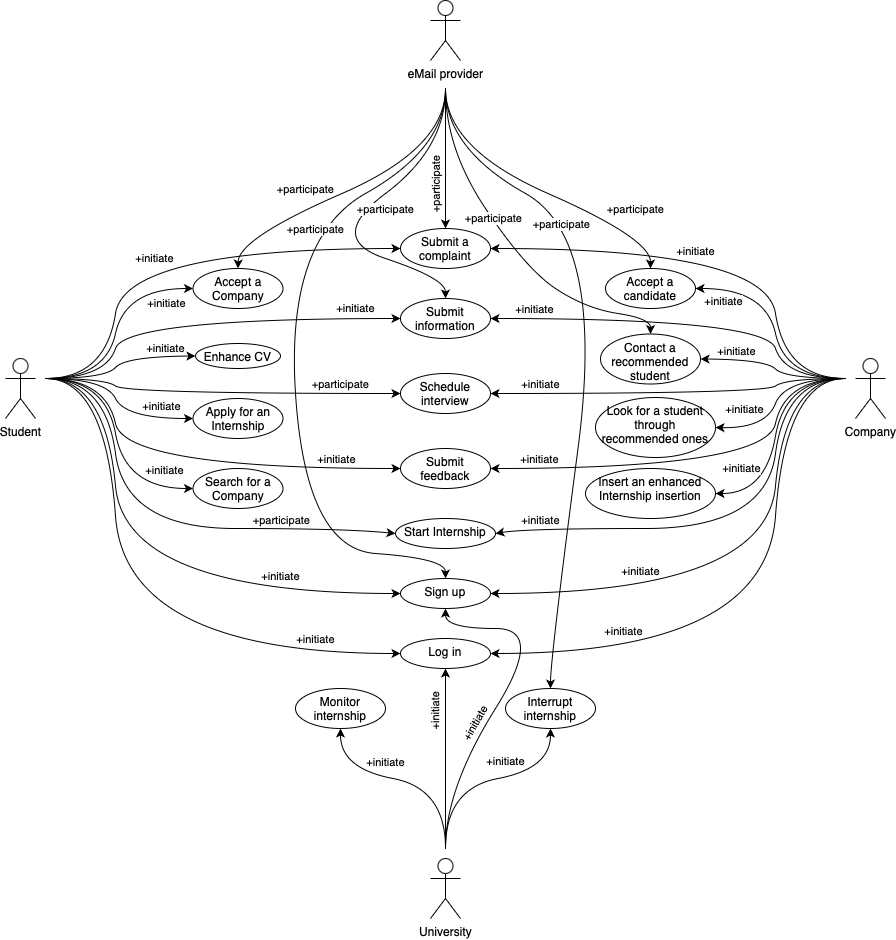
\includegraphics[width=6.5in,height=6.81319in]{Images/UCDiagram.png}
        \caption{Use Cases Diagram for all the Users.} 
        \label{fig:UnregisteredUC}%
        \end{center}
\end{figure}


\subsection{Use cases}
\label{subsec: use_cases}%
\newcounter{uc}
\setcounter{uc}{1}
\newcommand{\cuc}{\theuc\stepcounter{uc}}


\subsubsection*{UC\cuc . Sign Up}
\begin{center}
    \begin{longtable}{|l|p{0.75\linewidth}|}
        \hline
        \textbf{Name}               & Sign Up\\
        \hline
        \textbf{Actor}              & Guest, eMail provider\\
        \hline
        \textbf{Entry conditions}   & The Guest wants to create an account and knows the S\&C URL\\
        \hline
        \textbf{Event Flow}         & 1 - The Guest enters the URL of S\&C on the search bar of his browser.    \\
        & 2 - The Guest clicks on the “Sign Up” button entering in the registration page.    \\
        & 3 - The Guest selects the correct registration form by selecting the right option between Student, Company or University. \\
        & 4 - The Guest enters his personal information: eMail, password, name and username for the S; eMail, password, name, VAT Name and username for the C; eMail, password, name, PEC, Name and username for the U. \\
        & 5 - The Guest clicks on the “Accept \& Join” button.  \\
        & 6 - The system checks the credentials.    \\
        & 7 - If the check is successful the system sends a confirmation eMail to the User through the eMail provider.  \\
        \hline
        \textbf{Exit condition}   & The system lets the User enter the website. \\       
        \hline
        \textbf{Exceptions}       & \begin{itemize}
            \item The username is already in use, so the system shows an error message and the registration form is shown again.
            \item The eMail is already in use, so the system shows an error message and the registration form is shown again.
            \item The password is not valid: it’s less than 8 characters long and/or it doesn’t contain any uppercase letter and/or it doesn’t contain any lowercase letter and/or it doesn’t contain any number and/or it doesn’t contain any special character (!,\#,\&,\$,?,+,-). The system shows an error message and the registration form is shown again.
        \end{itemize}\\
        \hline
        \caption{Sign Up use case.}
        \label{tab: signup_as_ED_use_case}
    \end{longtable}
\end{center}


\subsubsection*{UC\cuc . Login}
\begin{center}
    \begin{longtable}{|l|p{0.75\linewidth}|}
        \hline
        \textbf{Name}               & Login\\
        \hline
        \textbf{Actor}              & Users\\
        \hline
        \textbf{Entry conditions}   & The Guest wants to access his account\\
        \hline
        \textbf{Event Flow}         & 
        1 - The Guest enters the URL of S\&C on the search bar of his browser.    \\
        2 - The Guest selects the right option between Student and Company button or in the case of a University clicks on the “Are you a University?” button. \\
        3 - The Guest enters the email and password in the correct form. \\
        4 - The Guest clicks on the “Login” button. \\
        5 - The system checks the credentials. If the check is successful it redirects the user to the right main page, according to his role.  \\
        \hline
        \textbf{Exit condition}   & The User is logged in and can surf into the website. \\       
        \hline
        \textbf{Exceptions}       & \begin{itemize}
            \item Incorrect eMail or password. An error message is shown and the User is redirected back to the Login page.
        \end{itemize}\\
        \hline
        \caption{Login use case.}
        \label{tab: login_use_case}
    \end{longtable}
\end{center}


\subsubsection*{UC\cuc . Insert an enhanced Internship Insertion}
\begin{center}
    \begin{longtable}{|l|p{0.75\linewidth}|}
        \hline
        \textbf{Name}               & Insert an enhanced Internship Insertion\\
        \hline
        \textbf{Actor}              & C\\
        \hline
        \textbf{Entry conditions}   & The C is logged in and wants to post a new insertion.\\
        \hline
        \textbf{Event Flow}         & 
        1 - The C goes to his profile page. \\
        2 - The C clicks on “Post”. \\
        3 - The C fills in the forms with all the information needed about his position. \\
        4 - The C clicks on the “Enhance” button. \\
        5 - The system analyzes the insertion and gives suggestions on how to improve project description. \\
        6 - The C reviews the suggestions given by the system and modifies the insertion if needed. \\
        7 - The C clicks on the “Post” button. \\
        \hline
        \textbf{Exit condition}   & The system publishes the C’s insertion and shows to the C his homepage. \\       
        \hline
        \textbf{Exceptions}       & \begin{itemize}
            \item The insertion is perfect and there aren’t any suggestions given.
        \end{itemize}\\
        \hline
        \caption{Insert an enhanced Internship Insertion use case.}
        \label{tab: enhanced_internship_insertion_use_case}
    \end{longtable}
\end{center}


\textbf{Figure \ldots..~ Insert an enhanced Internship insertion
sequence diagram}

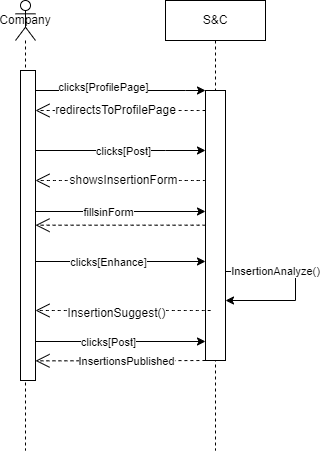
\includegraphics[width=4.44444in,height=6.26389in]{Images/image2.png}

\subsubsection*{UC\cuc . Enhance CV}
\begin{center}
    \begin{longtable}{|l|p{0.75\linewidth}|}
        \hline
        \textbf{Name}               & Enhance CV\\
        \hline
        \textbf{Actor}              & S\\
        \hline
        \textbf{Entry conditions}   & The S is logged in and wants to enhance his CV.\\
        \hline
        \textbf{Event Flow}         & 
        1 - The S opens his personal profile page. \\
        2 - The S scrolls down near the CV section. \\
        3 - The S clicks on the “Enhance” button. \\
        4 - The system analyzes the CV and gives suggestions on how to improve it. \\
        5 - The S reviews suggestions given by the system. \\
        6 - The S makes some suggested changes on the file of the CV. \\
        7 - The S reuploads a new version of CV. \\
        \hline
        \textbf{Exit condition}   & The system shows the S profile page. \\       
        \hline
        \textbf{Exceptions}       & \begin{itemize}
            \item The CV is perfect and there aren’t any suggestions given.
        \end{itemize}\\
        \hline
        \caption{Enhance CV use case.}
        \label{tab: enhance_cv_use_case}
    \end{longtable}
\end{center}
 

\textbf{Figure \ldots..~ Enhance Cv sequence diagram}

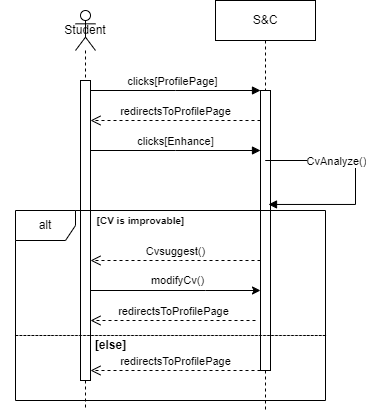
\includegraphics[width=5.08333in,height=5.70833in]{Images/image3.png}


\subsubsection*{UC\cuc . Submit a feedback}
\begin{center}
    \begin{longtable}{|l|p{0.75\linewidth}|}
        \hline
        \textbf{Name}               & Submit a feedback\\
        \hline
        \textbf{Actor}              & S, C\\
        \hline
        \textbf{Entry conditions}   & The S (C) wants to look for a recommended internship (student) and is logged in.\\
        \hline
        \textbf{Event Flow}         & 
        1 - The S (C) clicks on the home page. \\
        2 - The S (C) scrolls through the recommended insertions (students). \\
        3 - The S (C) clicks on a company’s insertion (student’s profile). \\
        4 - The system shows the review of the insertion (student). \\
        5 - The S (C) closes the window. \\
        6 - The system shows a pop-up asking the S (C) to submit a feedback, including rating and some comments on the received recommendations. \\
        7 - The S (C) submits his feedback. \\
        \hline
        \textbf{Exit condition}   & The system saves the feedback to feed the recommendation system and shows the homepage. \\       
        \hline
        \textbf{Exceptions}       & \begin{itemize}
            \item The system does not find any recommended C (S) available for the S (C).
        \end{itemize}\\
        \hline
        \caption{Submit a feedback use case.}
        \label{tab: submit_feedback_use_case}
    \end{longtable}
\end{center}


\textbf{Figure \ldots..~ Submit a feedback sequence diagram}

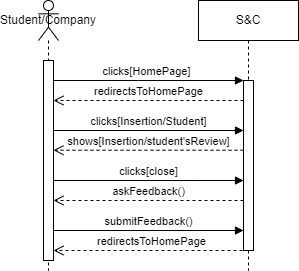
\includegraphics[width=5.11111in,height=4.625in]{Images/image4.png}

\subsubsection*{UC\cuc . Search for a company}
\begin{center}
    \begin{longtable}{|l|p{0.75\linewidth}|}
        \hline
        \textbf{Name}               & Search for a company\\
        \hline
        \textbf{Actor}              & S\\
        \hline
        \textbf{Entry conditions}   & The S is logged in and wants to search for a specific C.\\
        \hline
        \textbf{Event Flow}         & 
        1 - The S clicks on the home page. \\
        2 - The S clicks on the search bar. \\
        3 - The S writes the C’s name and clicks ‘Enter’ on the keyboard or the button ‘Search’. \\
        4 - The system shows a list of the matching results. \\
        5 - The S clicks on the C profile. \\
        \hline
        \textbf{Exit condition}   & The system shows the C profile. \\       
        \hline
        \textbf{Exceptions}       & \begin{itemize}
            \item The C isn’t registered on the platform.
        \end{itemize}\\
        \hline
        \caption{Search for a company use case.}
        \label{tab: search_for_a_company_use_case}
    \end{longtable}
\end{center}


\textbf{Figure \ldots..~ Search for a company~ sequence diagram}

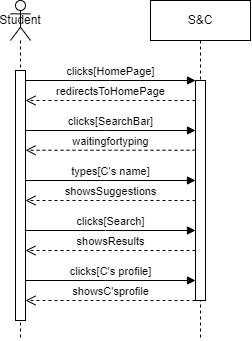
\includegraphics[width=5.63889in,height=7.625in]{Images/image5.png}

\subsubsection*{UC\cuc . Apply for an internship}
\begin{center}
    \begin{longtable}{|l|p{0.75\linewidth}|}
        \hline
        \textbf{Name}               & Apply for an internship\\
        \hline
        \textbf{Actor}              & S\\
        \hline
        \textbf{Entry conditions}   & The S is logged in and wants to apply for an internship.\\
        \hline
        \textbf{Event Flow}         & 
        1 - The S finds an interesting insertion. \\
        2 - The S clicks on the relative insertion. \\
        3 - The system shows the review of the insertion post. \\
        4 - The S applies for it, by clicking “Apply”. \\
        \hline
        \textbf{Exit condition}   & The system inserts S into the insertion’s candidates of the C. \\       
        \hline
        \textbf{Exceptions}       & \begin{itemize}
            \item No specific exceptions for this use case.
        \end{itemize}\\
        \hline
        \caption{Apply for an internship use case.}
        \label{tab: apply_for_an_internship_use_case}
    \end{longtable}
\end{center}


\textbf{Figure \ldots..~ Apply for a company~ sequence diagram}

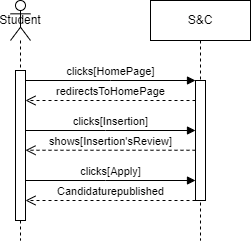
\includegraphics[width=3.5in,height=3.34722in]{Images/image6.png}


\subsubsection*{UC\cuc . Accept a candidate}
\begin{center}
    \begin{longtable}{|l|p{0.75\linewidth}|}
        \hline
        \textbf{Name}               & Accept a candidate\\
        \hline
        \textbf{Actor}              & C, eMail provider\\
        \hline
        \textbf{Entry conditions}   & The C is correctly logged in and wants to find a new candidate from the ones that applied for the internship.\\
        \hline
        \textbf{Event Flow}         & 
        1 - The C goes on his profile page. \\
        2 - The C clicks on the submitted insertion. \\
        3 - The system shows the review of the insertion. \\
        4 - The C opens the candidates’ section. \\
        5 - The C scrolls through all the possible candidates. \\
        6 - The C finds a S’s profile. \\
        7 - The C clicks on the S’s profile. \\
        8 - The system shows the S profile. \\
        9 - The C decides to accept the S’s profile by clicking on the “Accept” button. \\
        10 - The system sends an eMail to the S notifying him of the decision of the C through the eMail provider. \\
        \hline
        \textbf{Exit condition}   & The system creates a chat between the S and the C. \\       
        \hline
        \textbf{Exceptions}       & \begin{itemize}
            \item There are no candidates available for the internship.
        \end{itemize}\\
        \hline
        \caption{Accept a candidate use case.}
        \label{tab: accept_a_candidate_use_case}
    \end{longtable}
\end{center}


\textbf{Figure \ldots..~ Accept a candidate sequence diagram}

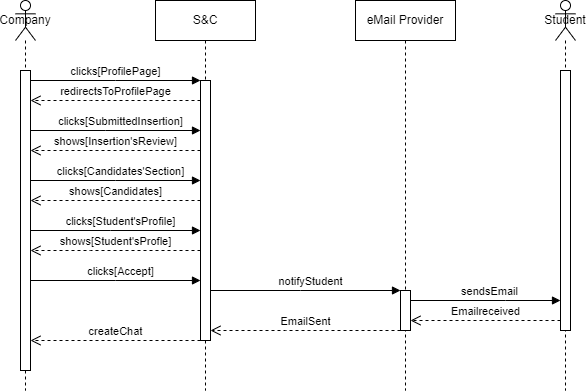
\includegraphics[width=6.5in,height=4.33681in]{Images/image7.png}


\subsubsection*{UC\cuc . Submit a Complaint}
\begin{center}
    \begin{longtable}{|l|p{0.75\linewidth}|}
        \hline
        \textbf{Name}               & Submit a Complaint\\
        \hline
        \textbf{Actor}              & S, C, eMail provider\\
        \hline
        \textbf{Entry conditions}   & The S (C) has encountered a problem during the internship period.\\
        \hline
        \textbf{Event Flow}         & 
        1 - The S (C) goes to the profile page. \\
        2 - The S (C) clicks on the chat section with the C (S). \\
        3 - The S (C) clicks on the “+” button. \\
        4 - The S (C) clicks on “Submit a Complaint”. \\
        5 - The system shows the user a form. \\
        6 - The S (C) describes the problem in the form. \\
        7 - The S (C) clicks on the “Submit” button. \\
        8 - The system checks if the insertion (description) is not empty. \\
        9 - If the problem insertion is not empty the system sends a notification and an eMail through the eMail provider to the S’s U. \\
        \hline
        \textbf{Exit condition}   & The complaint is submitted. \\       
        \hline
        \textbf{Exceptions}       & \begin{itemize}
            \item The user tried to submit an empty form. An error message is shown, inviting the user to describe the problem.
        \end{itemize}\\
        \hline
        \caption{Submit a Complaint use case.}
        \label{tab: submit_a_complaint_use_case}
    \end{longtable}
\end{center}


\subsubsection*{UC\cuc . Submit Information}
\begin{center}
    \begin{longtable}{|l|p{0.75\linewidth}|}
        \hline
        \textbf{Name}               & Submit Information\\
        \hline
        \textbf{Actor}              & S, C, eMail provider\\
        \hline
        \textbf{Entry conditions}   & The S (C) has some information to report regarding the ongoing internship.\\
        \hline
        \textbf{Event Flow}         & 
        1 - The S (C) goes to the profile page. \\
        2 - The S (C) clicks on the chat section with the C (S). \\
        3 - The S (C) clicks on the “+” button. \\
        4 - The S (C) clicks on “Submit an Information”. \\
        5 - The system shows the user a form. \\
        6 - The S (C) fills in the form. \\
        7 - The S (C) clicks on the “Submit” button. \\
        8 - The systems checks if the insertion is not null. \\
        9 - If the information insertion is not empty, the system sends a notification and an eMail through the eMail provider to the S’s U. \\
        \hline
        \textbf{Exit condition}   & The information is submitted. \\       
        \hline
        \textbf{Exceptions}       & \begin{itemize}
            \item The user tried to submit an empty form. An error message is shown, inviting the user to add the information in the form.
        \end{itemize}\\
        \hline
        \caption{Submit Information use case.}
        \label{tab: submit_information_use_case}
    \end{longtable}
\end{center}


\subsubsection*{UC\cuc . Look for a student through recommended ones}
\begin{center}
    \begin{longtable}{|l|p{0.75\linewidth}|}
        \hline
        \textbf{Name}               & Look for a student through recommended ones\\
        \hline
        \textbf{Actor}              & C\\
        \hline
        \textbf{Entry conditions}   & The C wants to look for a S and has an open position for an internship.\\
        \hline
        \textbf{Event Flow}         & 
        1 - The C clicks on the profile page. \\
        2 - The C selects the internship posting for which it wants to find a candidate. \\
        3 - The C starts scrolling through the recommended student’s profiles. \\
        \hline
        \textbf{Exit condition}   & The C changes page. \\       
        \hline
        \textbf{Exceptions}       & \begin{itemize}
            \item There are no recommended S for that internship posting.
        \end{itemize}\\
        \hline
        \caption{Look for a student through recommended ones use case.}
        \label{tab: look_for_student_use_case}
    \end{longtable}
\end{center}


\subsubsection*{UC\cuc . Contact a recommended student}
\begin{center}
    \begin{longtable}{|l|p{0.75\linewidth}|}
        \hline
        \textbf{Name}               & Contact a recommended student\\
        \hline
        \textbf{Actor}              & C, eMail provider\\
        \hline
        \textbf{Entry conditions}   & The C wants to send the proposal for an internship to a recommended student.\\
        \hline
        \textbf{Event Flow}         & 
        1 - The C clicks on the profile page. \\
        2 - The C selects the internship posting for which it wants to find a candidate. \\
        3 - The C starts scrolling through the recommended student’s profiles. \\
        4 - The C clicks on the profile of a recommended S. \\
        5 - The C reviews the S’s CV. \\
        6 - The C contacts the S, by clicking “Contact”. \\
        7 - The system sends a notification and an eMail through the eMail provider to the S. \\
        \hline
        \textbf{Exit condition}   & The S receives a contact request from the C. \\       
        \hline
        \textbf{Exceptions}       & \begin{itemize}
            \item There are no recommended students for the internship.
        \end{itemize}\\
        \hline
        \caption{Contact a recommended student use case.}
        \label{tab: contact_recommended_student_use_case}
    \end{longtable}
\end{center}


\subsubsection*{UC\cuc . Accept a company}
\begin{center}
    \begin{longtable}{|l|p{0.75\linewidth}|}
        \hline
        \textbf{Name}               & Accept a company\\
        \hline
        \textbf{Actor}              & S, eMail provider\\
        \hline
        \textbf{Entry conditions}   & The C has contacted the S proposing him an internship position and the S wants to accept it.\\
        \hline
        \textbf{Event Flow}         & 
        1 - The S goes on his profile page. \\
        2 - The S clicks on the notifications button. \\
        3 - The S scrolls through the list of C that contacted him. \\
        4 - The S clicks on the C’s profile and reviews the internship description. \\
        5 - The S decides to accept the internship by clicking on the “Accept” button. \\
        6 - An email is sent to the C through the eMail provider, notifying them that the student accepted their request. \\
        \hline
        \textbf{Exit condition}   & The system creates a chat between the S and the C. \\       
        \hline
        \textbf{Exceptions}       & None. \\
        \hline
        \caption{Accept a company use case.}
        \label{tab: accept_company_use_case}
    \end{longtable}
\end{center}


\subsubsection*{UC\cuc . Interrupt internship}
\begin{center}
    \begin{longtable}{|l|p{0.75\linewidth}|}
        \hline
        \textbf{Name}               & Interrupt internship\\
        \hline
        \textbf{Actor}              & U, eMail provider\\
        \hline
        \textbf{Entry conditions}   & The U monitors the internship and reads a complaint.\\
        \hline
        \textbf{Event Flow}         & 
        1 - The U goes on the main page. \\
        2 - The U clicks on the related chat. \\
        3 - The U reviews the complaint. \\
        4 - If the U deems it necessary, clicks on “Interrupt Internship”. \\
        5 - The system sends an eMail through the eMail provider and notifies the S and C about the interruption of the internship. \\
        \hline
        \textbf{Exit condition}   & The internship is interrupted and the chat closed. \\       
        \hline
        \textbf{Exceptions}       & None. \\
        \hline
        \caption{Interrupt internship use case.}
        \label{tab: interrupt_internship_use_case}
    \end{longtable}
\end{center}


\subsubsection*{UC\cuc . Monitor internship}
\begin{center}
    \begin{longtable}{|l|p{0.75\linewidth}|}
        \hline
        \textbf{Name}               & Monitor internship\\
        \hline
        \textbf{Actor}              & U\\
        \hline
        \textbf{Entry conditions}   & The U monitors the internship between the C and the S.\\
        \hline
        \textbf{Event Flow}         & 
        1 - The U goes on the main page. \\
        2 - The U clicks on the chat regarding the S and the C. \\
        3 - The system shows the chat and the related complaints or information. \\
        \hline
        \textbf{Exit condition}   & The U can monitor the information and issues reported by the other two parties during the internship. \\       
        \hline
        \textbf{Exceptions}       & None. \\
        \hline
        \caption{Monitor internship use case.}
        \label{tab: monitor_internship_use_case}
    \end{longtable}
\end{center}


\subsubsection*{UC\cuc . Schedule an Interview}
\begin{center}
    \begin{longtable}{|l|p{0.75\linewidth}|}
        \hline
        \textbf{Name}               & Schedule an Interview\\
        \hline
        \textbf{Actor}              & S, C\\
        \hline
        \textbf{Entry conditions}   & The S and the C have accepted each other’s request and a chat is established between them.\\
        \hline
        \textbf{Event Flow}         & 
        1 - The C clicks on the “+” button. \\
        2 - The C selects “schedule interview”. \\
        3 - The C compiles a form selecting a date and time for the interview. \\
        4 - The C submits the form and sends it to the S. \\
        5 - The S can either accept or decline the proposal by selecting the appropriate option. \\
        6 - If the S accepts, the event is added to the S\&C calendar for both the S and the C. \\
        \hline
        \textbf{Exit condition}   & An interview event is scheduled and added to both the S’s and the C’s S\&C calendars. \\       
        \hline
        \textbf{Exceptions}       & The S declines the interview proposal from the C. \\
        \hline
        \caption{Schedule an Interview use case.}
        \label{tab: schedule_interview_use_case}
    \end{longtable}
\end{center}


\subsubsection*{UC\cuc . Start an Internship}
\begin{center}
    \begin{longtable}{|l|p{0.75\linewidth}|}
        \hline
        \textbf{Name}               & Start an Internship\\
        \hline
        \textbf{Actor}              & S, C\\
        \hline
        \textbf{Entry conditions}   & The S and the C have already completed an interview, and the C is impressed with the S.\\
        \hline
        \textbf{Event Flow}         & 
        1 - The C clicks on the “+” button. \\
        2 - The C selects “propose internship”. \\
        3 - The S accepts the proposal by selecting the appropriate option. \\
        \hline
        \textbf{Exit condition}   & The system adds a “starting internship” to both the S’s and the C’s S\&C calendars. \\       
        \hline
        \textbf{Exceptions}       & The S declines the offer and the chat between S and C is closed. \\
        \hline
        \caption{Start an Internship use case.}
        \label{tab: start_internship_use_case}
    \end{longtable}
\end{center}


\subsection{Mapping on goals}
\label{subsec:mapping_on_goals}%

The mapping links the platform's goals to specific
requirements and domain assumptions, ensuring each objective is
addressed effectively.

\begin{itemize}
\item
  \textbf{{[}G1{]}: University students would like to seek internships
  that better align with their interests and field of study.}

  \begin{itemize}
  \item
    {[}R1{]}: The system should allow an unregistered guest to sign up.
  \item
    {[}R2{]}: The system should allow registered students to log in.
  \item
    {[}R3{]}: The system should allow students to insert their CVs and
    manage their profile information (e.g. personal data, skills and
    profile photo).
  \item
    {[}R4{]}: The system should provide personalized suggestions to
    students for enhancing their CVs to improve their chances of being
    selected.
  \item
    {[}R5{]}: The system should notify students when internships
    matching their skills, experiences, and interests become available.
  \item
    {[}R6{]}: The system should allow students to browse available
    internship postings.
  \item
    {[}R7{]}: The system allows S to visualize the profile of other C.~
  \item
    {[}R8{]}: The system should allow S to submit applications for
    specific internship postings.
  \item
    {[}D1{]} S must be enrolled in a U.
  \item
    {[}D3{]} S should already have a valid Cv to be uploaded.
  \item
    {[}D4{]} S's Cv should be a PDF document.
  \item
    {[}D5{]} The User can easily access his eMail provider.
  \item
    {[}D6{]} S,C provide accurate and truthful information in their
    profiles, CVs, and internship description.
  \item
    {[}D9{]} The S\&C recommendation engine achieves high accuracy when
    S and C provide detailed, complete, and accurate information in
    their CVs and job descriptions.
  \item
    {[}D10{]} The AI system integrated into the S\&C platform
    effectively enhances students' CVs and
    companies' internship postings, providing accurate
    and useful suggestions to improve the matching process.
  \item
    {[}D11{]} The eMail provider functions reliably, ensuring that all
    emails, including verification and notification messages, are
    successfully delivered to the intended recipients.
  \end{itemize}
\end{itemize}

\begin{itemize}
\item
  \textbf{{[}G2{]}: Companies would like to offer internships to
  students who best match the related figure.}

  \begin{itemize}
  \item
    {[}R1{]}: The system should allow an unregistered guest to sign up.
  \item
    {[}R16{]}: The system should allow registered companies to log in.
  \item
    {[}R17{]}: The system should allow C to manage their organization
    profile.
  \item
    {[}R18{]}: The system should allow C to post new internship
    opportunities, specifying details such as required skills, tasks,
    and benefits.
  \item
    {[}R19{]}: The system should provide suggestions to C to improve
    their internship postings, making them more appealing to S.
  \item
    {[}R20{]}: The system allows C to visualize the profile of other
    Users.
  \item
    {[}R21{]}: The system should inform C about the availability of S
    CVs corresponding to their needs.
  \item
    {[}R23{]}: The system allows C to establish a contact with S when
    mutual interest is identified.
  \item
    {[}D5{]} The User can easily access his eMail provider.
  \item
    {[}D6{]} S,C provide accurate and truthful information in their
    profiles, CVs, and internship description.
  \item
    {[}D8{]} C on the platform are assumed to be legitimate and offer
    genuine internships, operating legally and ethically without
    verification by S\&C.
  \item
    {[}D9{]} The S\&C recommendation engine achieves high accuracy when
    S and C provide detailed, complete, and accurate information in
    their CVs and job descriptions.
  \item
    {[}D10{]} The AI system integrated into the S\&C platform
    effectively enhances students' CVs and
    companies' internship postings, providing accurate
    and useful suggestions to improve the matching process.
  \item
    {[}D11{]} The eMail provider functions reliably, ensuring that all
    emails, including verification and notification messages, are
    successfully delivered to the intended recipients.
  \end{itemize}
\end{itemize}

\begin{itemize}
\item
  \textbf{{[}G3{]}: Enhance communication and coordination between
  students and companies in the selection process.}

  \begin{itemize}
  \item
    {[}R2{]}: The system should allow registered students to log in.
  \item
    {[}R10{]}: The system allows S to establish a contact with C when
    mutual interest is identified.
  \item
    {[}R11{]}: The system should assist S in scheduling interviews.
  \item
    {[}R12{]}: The system should allow S to track the status of their
    applications and final selections.
  \item
    {[}R14{]}: The system should allow S to review the S\&C Calendar.
  \item
    {[}R15{]}: The system should insert the S's events on the S\&C
    Calendar.
  \item
    {[}R16{]}: The system should allow registered companies to log in.
  \item
    {[}R23{]}: The system allows C to establish a contact with S when
    mutual interest is identified.
  \item
    {[}R24{]}: The system should enable C to track the progress of their
    internship selection processes, including applications and
    decisions.~
  \item
    {[}R26{]}: The system should allow C to review the S\&C Calendar.
  \item
    {[}R27{]}: The system should insert the C's events on the S\&C
    Calendar.
  \item
    {[}D12{]} Students and companies are committed to the internship
    process and will engage with features such as scheduling interviews
    and responding to feedback.
  \item
    {[}D13{]} Companies must clearly communicate interview requirements
    (e.g., time, format, platform) to students during scheduling.
  \item
    {[}D14{]} Interviews must be conducted either in person or via
    secure external tools, with students and companies responsible for
    ensuring their availability and functionality.
  \end{itemize}
\end{itemize}

\begin{itemize}
\item
  \textbf{{[}G4{]}: Evolve the recommendation system through feedback
  and suggestions (provided by students and companies) to improve future
  matches.}

  \begin{itemize}
  \item
    {[}R2{]}: The system should allow registered students to log in.
  \item
    {[}R5{]}: The system should notify students when internships
    matching their skills, experiences, and interests become available.
  \item
    {[}R7{]}: The system allows S to visualize the profile of other C.~
  \item
    {[}R9{]}: The system should allow S to provide feedback, suggestions
    and rating to improve the recommendation process.
  \item
    {[}R16{]}: The system should allow registered companies to log in.
  \item
    {[}R20{]}: The system allows C to visualize the profile of other
    Users.
  \item
    {[}R21{]}: The system should inform C about the availability of S
    CVs corresponding to their needs.
  \item
    {[}R22{]}: The system should allow C to provide feedback and
    suggestions to improve the recommendation process.
  \item
    {[}D6{]} S,C provide accurate and truthful information in their
    profiles, CVs, and internship description.
  \item
    {[}D9{]} The S\&C recommendation engine achieves high accuracy when
    S and C provide detailed, complete, and accurate information in
    their CVs and job descriptions.
  \item
    {[}D10{]} The AI system integrated into the S\&C platform
    effectively enhances students' CVs and
    companies' internship postings, providing accurate
    and useful suggestions to improve the matching process.
  \item
    {[}D12{]} Students and companies are committed to the internship
    process and will engage with features such as scheduling interviews
    and responding to feedback.
  \end{itemize}
\end{itemize}

\begin{itemize}
\item
  \textbf{{[}G5{]}: Universities would like to monitor internships and
  handle any emerging issues promptly, ensuring a smooth and beneficial
  experience for all parties involved.}

  \begin{itemize}
  \item
    {[}R1{]}: The system should allow an unregistered guest to sign up.
  \item
    {[}R13{]}: The system should provide S with a mechanism to report
    issues or complaints related to ongoing internships.
  \item
    {[}R25{]}: The system should allow C to submit complaints or
    information related to internships.
  \item
    {[}R28{]}: The system should allow U to log in.
  \item
    {[}R29{]}: The system should allow U to monitor internships of their
    students.
  \item
    {[}R30{]}: The system should allow U to interrupt ongoing
    internships.
  \item
    {[}D2{]} The related U should be already registered when the S signs
    up.
  \item
    {[}D5{]} The User can easily access his eMail provider.
  \item
    {[}D7{]} U are willing and able to use the S\&C platform to monitor
    internship statuses, address complaints, and respond to student or
    company feedback as needed.
  \item
    {[}D11{]} The eMail provider functions reliably, ensuring that all
    emails, including verification and notification messages, are
    successfully delivered to the intended recipients.
  \end{itemize}
\end{itemize}

\begin{longtable}[]{@{}
  >{\raggedright\arraybackslash}p{(\columnwidth - 12\tabcolsep) * \real{0.5858}}
  >{\raggedright\arraybackslash}p{(\columnwidth - 12\tabcolsep) * \real{0.0656}}
  >{\raggedright\arraybackslash}p{(\columnwidth - 12\tabcolsep) * \real{0.0656}}
  >{\raggedright\arraybackslash}p{(\columnwidth - 12\tabcolsep) * \real{0.0656}}
  >{\raggedright\arraybackslash}p{(\columnwidth - 12\tabcolsep) * \real{0.0656}}
  >{\raggedright\arraybackslash}p{(\columnwidth - 12\tabcolsep) * \real{0.0656}}
  >{\raggedright\arraybackslash}p{(\columnwidth - 12\tabcolsep) * \real{0.0861}}@{}}
\toprule()
\begin{minipage}[b]{\linewidth}\raggedright
\textbf{Requirements and Domain Assumption}
\end{minipage} & \begin{minipage}[b]{\linewidth}\raggedright
\textbf{G1}
\end{minipage} & \begin{minipage}[b]{\linewidth}\raggedright
\textbf{G2}
\end{minipage} & \begin{minipage}[b]{\linewidth}\raggedright
\textbf{G3}
\end{minipage} & \begin{minipage}[b]{\linewidth}\raggedright
\textbf{G4}
\end{minipage} & \begin{minipage}[b]{\linewidth}\raggedright
\textbf{G5}
\end{minipage} & \begin{minipage}[b]{\linewidth}\raggedright
\textbf{UC}
\end{minipage} \\
\midrule()
\endhead
R1 & X & X & & & X & UC1 \\
R2 & X & & X & X & & UC2 \\
R3 & X & & & & & \\
R4 & X & & & & & \\
R5 & X & & & X & & \\
R6 & X & & & & & \\
R7 & X & & & X & & \\
R8 & X & & & & & \\
R9 & & & & X & & \\
R10 & & & X & & & \\
R11 & & & X & & & \\
R12 & & & X & & & \\
R13 & & & & & X & \\
R14 & & & X & & & \\
R15 & & & X & & & \\
R16 & & X & X & X & & UC2 \\
R17 & & X & & & & \\
R18 & & X & & & & \\
R19 & & X & & & & \\
R20 & & X & & X & & \\
R21 & & X & & X & & \\
R22 & & & & X & & \\
R23 & & X & X & & & \\
R24 & & & X & & & \\
R25 & & & & & X & \\
R26 & & & X & & & \\
R27 & & & X & & & \\
R28 & & & & & X & \\
R29 & & & & & X & \\
R30 & & & & & X & \\
D1 & X & & & & & \\
D2 & & & & & X & \\
D3 & X & & & & & \\
D4 & X & & & & & \\
D5 & X & X & & & X & \\
D6 & X & X & & X & & \\
D7 & & & & & X & \\
D8 & & X & & & & \\
D9 & X & X & & X & & \\
D10 & X & X & & X & & \\
D11 & X & X & & & X & \\
D12 & & & X & X & & \\
D13 & & & X & & & \\
D14 & & & X & & & \\
\bottomrule()
\end{longtable}

Traceability Matrix for Goals and related Requirements~

and Domain Assumptions


\section{Performance requirements}
\label{sec:performance_requirements}%


\paragraph{Number of Concurrent Users:}
  The S\&C platform must be designed to handle a significant number of
  concurrent users, ensuring smooth performance even during peak
  activity periods, such as internship application deadlines. The
  platform should support a substantial portion of its active user base
  accessing the system simultaneously.
\paragraph{Data Storage:}
  The platform must store and manage all relevant information about
  students, including CVs, profiles, and application statuses, as well
  as companies' internship postings, feedback, and selection processes.
  Historical data, such as completed internships and feedback, should
  remain accessible to support recommendations and user references.
\paragraph{Response Time:}
  Operations directly executed by the S\&C platform, such as
  registration, login, posting internships, applying for internships,
  and scheduling interviews, must have a response time of under 500
  milliseconds. For operations involving external systems, such as email
  notifications or third-party scheduling tools, the platform will
  strive to minimize delays but cannot guarantee their performance.

\section{Design constraints}
\label{sec:design_constraints}%


\subsection{Standard compliance}
\label{subsec:standard compliance}%%


The S\&C platform must comply with relevant data protection and privacy
regulations, including the EU's General Data Protection Regulation
(GDPR). This regulation ensures that the personal data of users,
including students, companies, and universities, is collected, stored,
and processed securely and transparently. The platform must implement
appropriate measures to protect user privacy and ensure data security.


\subsection{Hardware limitations}
\label{subsec:hardware_limitations}%


The primary hardware requirement for accessing the S\&C platform is a
reliable internet connection and a device with a modern web browser.


\section{Software system attributes}
\label{sec:software_system_attributes}%


\subsection{Reliability}
\label{subsec:reliability}%


The S\&C platform must be fault-tolerant to ensure continuous service
and minimize the impact of potential errors. This will prevent system
failures from propagating, allowing users to continue their tasks
without significant interruptions.


\subsection{Availability}
\label{subsec:availability}%


The S\&C platform must maintain a high level of availability. This
ensures that the platform is accessible to users at all times,
minimizing disruption to their internship search and application
processes.~


\subsection{Security}
\label{subsec:security}%


The platform must implement robust security measures to protect user
data and ensure secure access. This includes both authentication and
authorization:

\begin{itemize}
\item
  Authentication will verify the identity of users attempting to log in,
  ensuring only legitimate users can access the platform.
\item
  Authorization will manage the permissions of authenticated users,
  restricting access to specific features based on user roles (e.g.,
  students, companies, or universities).
\end{itemize}

To protect sensitive information, the system will adopt best practices
for data security, including:

\begin{itemize}
\item
  Encryption of passwords and personal data stored in the database.
\item
  Protection against query injections and other common security
  vulnerabilities to prevent unauthorized data access.
\end{itemize}

These measures will ensure that the system maintains a secure
environment for users and their data.


\subsection{Maintainability}
\label{subsec:maintainability}%


The S\&C platform must be designed using scalable and modular components
to allow easy updates and additions of new features with minimal effort.
The architecture should support future expansions, such as new
functionalities or integrations with third-party services, without major
changes to the core system. Regular maintenance should be scheduled
during off-peak hours, preferably at night, to ensure minimal disruption
to users during peak traffic periods.


\subsection{Portability}
\label{subsec:portability}%


The system must be accessible to users from any device or platform that
supports a modern web browser. This ensures that students, companies,
and universities can access the platform from a variety of devices. On
the server side, there are no specific portability requirements, as the
platform will rely on standard web technologies and services to ensure
compatibility across different environments.


    \chapter{Formal Analysis Using Alloy}
    \label{ch:formal_analysis_alloy}%
    In this section is presented the detailed alloy specification for the system, as outlined and described in the RASD.
\vspace{2cm}
\lstinputlisting[language=alloy]{Alloy/Alloy.als}
\newpage


    \chapter{Effort Spent}
    \label{ch:effort_spent}%
    \begin{table}[H]
    \begin{center}
        \begin{tabular}{|c|c|}
            \hline
            Member of group & Effort spent \\
            \hline
            De Matteis Alessandro & \begin{tabular}{p{0.25\linewidth}|c}
                            Introduction          & $h$ \\
                            Overall description   & $h$ \\
                            Specific requirements & $h$ \\
                            Formal analysis       & $h$ \\
                            Logic Development     & $h$ \\
            \end{tabular} \\
            \hline
            Marino Margherita & \begin{tabular}{p{0.25\linewidth}|c}
                            Introduction          & $h$ \\
                            Overall description   & $h$ \\
                            Specific requirements & $h$ \\
                            Formal analysis       & $h$ \\
                            Logic Development     & $h$ \\
            \end{tabular} \\
            \hline
            Monaco Giorgio & \begin{tabular}{p{0.25\linewidth}|c}
                            Introduction          & $h$ \\
                            Overall description   & $h$ \\
                            Specific requirements & $h$ \\
                            Formal analysis       & $h$ \\
                            Logic Development     & $h$ \\
            \end{tabular} \\
            \hline
        \end{tabular}
        \caption{Effort spent by each member of the group.}
        \label{tab:effor_spent}
    \end{center}
\end{table}


    \chapter{References}
    \label{ch:references}%
    \section{References}
\label{sec:references}%

\begin{itemize}
    \item 29148-2018 - ISO/IEC/IEEE International Standard - Systems and software engineering - Life cycle processes - Requirements engineering.
    \item A.Y. 2024-2025 Software Engineering 2 Requirement Engineering and Design Project.
\end{itemize}

\section{Used Tools}
\label{sec:used_tools}%
\begin{itemize}
    \item \textit{GitHub} for project versioning and sharing.
    \item \LaTeX{} and \textit{Overleaf} as editor for writing this document.
    \item \textit{draw.io} for all the diagrams' design.
    \item \textit{figma} for the UI's design.
    \item \textit{Alloy Analyzer 6.1.0} for formal analysis.
    \item \textit{Google Documents} for collaborative writing, notes and reasoning.
\end{itemize}


% LIST OF FIGURES
    \listoffigures
    
% LIST OF TABLES
    \listoftables
    \cleardoublepage

\end{document}
